% ============================================================
% strategy_body.tex — Research Strategy
% NIH R03 limit: 6 pages (references are excluded and do NOT count)
%
% Standard NIH structure: A. Significance → B. Innovation → C. Approach
% Subsection numbering is conventional but not required by NIH.
% All \cite{} calls here resolve from proposal_package.tex bibliography.
% ============================================================

{\noindent\fontsize{12}{14}\selectfont\bfseries RESEARCH STRATEGY}

\medskip

% ============================================================
\section*{A. SIGNIFICANCE}
% ============================================================

\subsection*{A.1 \placeholder{Problem statement subsection title}}

\placeholder{Describe the target condition, population, or scientific problem.
Establish prevalence/burden with citations. Describe the clinical or scientific
importance. Explain what is currently not understood or not possible.
3--5 sentences.}\cite{placeholder}

\subsection*{A.2 \placeholder{Knowledge gap subsection title}}

\placeholder{Describe the key barrier to progress. This may be a data gap,
methodological limitation, or lack of an appropriate tool or resource.
Be specific about what is missing and why existing approaches fall short.
3--4 sentences.}\cite{placeholder}

\subsection*{A.3 \placeholder{Enabling opportunity subsection title}}

\placeholder{Describe the specific resource, technology, or data source that
now makes this work possible. Explain why this opportunity is timely.
2--3 sentences.}\cite{placeholder}

\subsection*{A.4 Significance of the expected contribution}

\placeholder{State the critical need this project addresses. Describe what
the field will be able to do after this project that it cannot do now.
Connect to the funding priority or NIH strategic goal. 2--3 sentences.}

% ============================================================
\section*{B. INNOVATION}
% ============================================================

This project is innovative along \placeholder{N} distinct dimensions:

\textbf{B.1 \placeholder{Innovation 1 label.}} \placeholder{Describe what
is new about the approach, resource, or method. Contrast with prior work.
2--3 sentences.}

\textbf{B.2 \placeholder{Innovation 2 label.}} \placeholder{Describe the
second innovative dimension. 2--3 sentences.}

\textbf{B.3 \placeholder{Innovation 3 label.}} \placeholder{Describe the
third innovative dimension. 2--3 sentences.}

\textbf{B.4 \placeholder{Innovation 4 label (optional).}} \placeholder{Describe
reusability, generalizability, or infrastructure innovation. 2--3 sentences.}

% ============================================================
\section*{C. APPROACH}
% ============================================================

\subsection*{C.1 Research team}

\placeholder{Describe the team's collective expertise and how it maps to the
aims. For MPI submissions, note the Leadership Plan attachment. Name each
investigator and their key qualification. Include institutional resources
(computing, data governance, IRB) that support feasibility. 2--3 paragraphs.}

\subsection*{C.2 Preliminary studies}

\placeholder{Describe prior work by the team that directly supports
feasibility. Connect each preliminary finding to a specific aim or
methodological choice. If preliminary data are limited (as is common for
pilot/R03 applications), describe conceptual or methodological groundwork.
2--3 paragraphs.}

\subsection*{C.3 Project design and framework}

\placeholder{Provide a brief overview of the overall study design and
conceptual framework. State the number of phases or aims and how they
build on each other. Include a figure if it aids comprehension.}

% ---- OVERVIEW FIGURE (optional — delete if not needed) ----
\begin{figure}[ht]
\centering
\resizebox{\textwidth}{!}{%
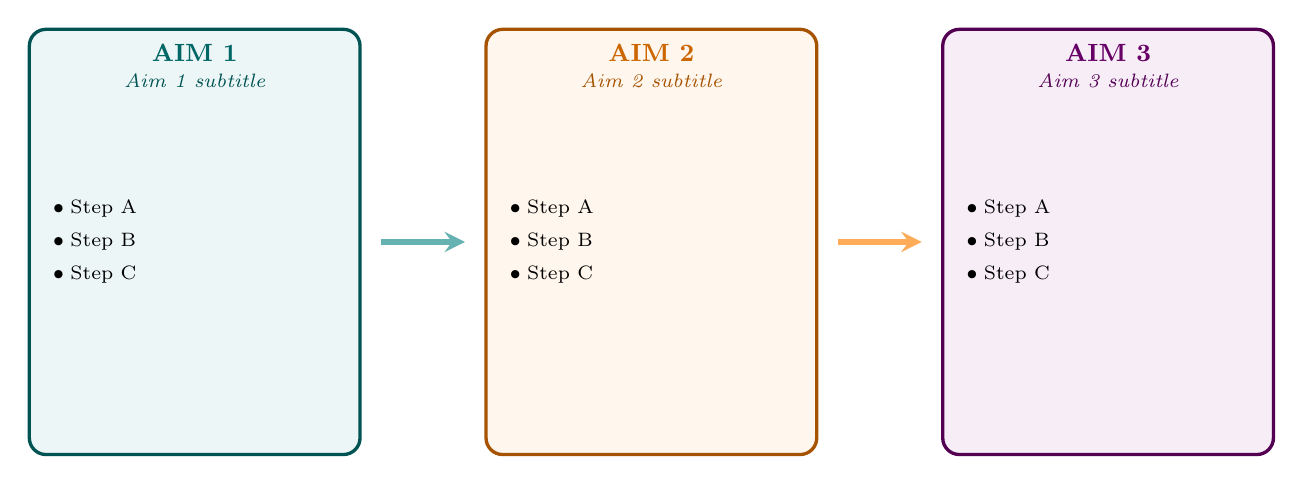
\begin{tikzpicture}[
  font=\small, >=stealth,
  pnl/.style  = {rounded corners=6pt, draw, very thick,
                 minimum width=4.2cm, minimum height=5.4cm, inner sep=0pt},
  phdr/.style = {font=\small\bfseries, align=center},
  psub/.style = {font=\scriptsize\itshape},
  pit/.style  = {align=left, font=\scriptsize, text width=3.6cm},
  arr/.style  = {->, line width=2.2pt, shorten >=7pt, shorten <=7pt},
]

%% Panel 1 — Aim 1
\node[pnl, fill=teal!7, draw=teal!65!black] (P1) at (0, 0) {};
\node[phdr, teal!80!black] at (0, 2.4) {AIM 1};
\node[psub, teal!65!black] at (0, 2.05) {\placeholder{Aim 1 subtitle}};
\node[pit] at (0, 0) {
  $\bullet$\;\placeholder{Step A}\\[4pt]
  $\bullet$\;\placeholder{Step B}\\[4pt]
  $\bullet$\;\placeholder{Step C}
};

%% Panel 2 — Aim 2
\node[pnl, fill=orange!7, draw=orange!65!black] (P2) at (5.8, 0) {};
\node[phdr, orange!80!black] at (5.8, 2.4) {AIM 2};
\node[psub, orange!65!black] at (5.8, 2.05) {\placeholder{Aim 2 subtitle}};
\node[pit] at (5.8, 0) {
  $\bullet$\;\placeholder{Step A}\\[4pt]
  $\bullet$\;\placeholder{Step B}\\[4pt]
  $\bullet$\;\placeholder{Step C}
};

%% Panel 3 — Aim 3
\node[pnl, fill=violet!7, draw=violet!65!black] (P3) at (11.6, 0) {};
\node[phdr, violet!80!black] at (11.6, 2.4) {AIM 3};
\node[psub, violet!65!black] at (11.6, 2.05) {\placeholder{Aim 3 subtitle}};
\node[pit] at (11.6, 0) {
  $\bullet$\;\placeholder{Step A}\\[4pt]
  $\bullet$\;\placeholder{Step B}\\[4pt]
  $\bullet$\;\placeholder{Step C}
};

%% Arrows
\draw[->, line width=2.2pt, teal!60, shorten >=7pt, shorten <=7pt]
  (P1.east) -- (P2.west);
\draw[->, line width=2.2pt, orange!65, shorten >=7pt, shorten <=7pt]
  (P2.east) -- (P3.west);

\end{tikzpicture}%
}
\caption{\textbf{Project Overview.} \placeholder{One-sentence figure caption.}}
\label{fig:overview}
\end{figure}

\subsection*{C.4 Data sources}

\placeholder{Describe each data source: name, scope, variables of interest,
and how CP/cancer (or your target condition) is identified (e.g., ICD codes,
registry criteria). State access pathway for any restricted data (dbGaP, DUA,
IRB). Note which sources can be accessed immediately vs.\ at award initiation.
Use numbered list or short paragraphs per source.}

\subsection*{C.5 Data analysis}

\textbf{C.5.1 Analytic plan for Aim 1.}
\placeholder{Describe the statistical or computational methods for Aim 1.
Name specific models, algorithms, or tools. Describe expected inputs and
outputs. State evaluation criteria used to select among competing approaches.
Use underlined subheadings for major methodological steps if helpful.
3--5 sentences per major step.}

\textbf{C.5.2 Analytic plan for Aim 2.}
\placeholder{Describe the statistical or computational methods for Aim 2.
Include pre-specified thresholds or benchmarks where applicable. Describe
the validation or testing approach and what constitutes success.
3--5 sentences per major step.}

\textbf{C.5.3 Analytic plan for Aim 3.}
\placeholder{Describe the dissemination, workflow development, or deployment
plan for Aim 3. Specify deliverables (code, cohorts, documentation, portal).
Name the repositories, DOI mechanisms, and presentation venues.
3--5 sentences per major step.}

\subsection*{C.6 Methodological Issues and Opportunities}

\placeholder{Describe 3--4 potential methodological problems and your
mitigation strategy for each. Use a consistent structure: (1) state the risk,
(2) explain why it matters, (3) describe the specific mitigation approach and
fallback plan. This section demonstrates rigor — reviewers look for it.
1 paragraph per issue.}

\subsection*{C.7 Timeline}

Conducting this study is feasible within \placeholder{N} year(s) (Table~1).
\placeholder{1--2 sentences on team readiness and why key milestones
are achievable within the proposed period.}

% ---- GANTT CHART ----
% Update {START-YYYY-MM}{END-YYYY-MM} and task dates to match your project.
% All dates must use YYYY-MM format with the isodate-yearmonth slot format.
% Milestone diamond size is controlled by milestone left/right shift — do not change.
\begingroup
\renewcommand{\figurename}{Table}
\setcounter{figure}{0}
\begin{figure}[h]
  \caption{\textbf{Study Timeline}}
  \label{fig:gantt}
  \centering
  \resizebox{\textwidth}{!}{%
    \begin{ganttchart}[
      vgrid,
      hgrid,
      y unit title     = 0.46cm,
      y unit chart     = 0.37cm,
      time slot format = isodate-yearmonth,
      time slot unit   = month,
      x unit           = 1.32cm,
      title height     = 1,
      bar height       = 0.58,
      bar top shift    = 0.21,
      milestone left shift  = .5,
      milestone right shift = -.5,
      milestone top shift   = 0.21,
      milestone height      = 0.58,
      bar/.append style       = {rounded corners=1.5pt},
      milestone/.append style = {shape=regular polygon, regular polygon sides=4,
                                  rotate=45, inner sep=0pt},
      bar label font          = \scriptsize,
      title label font        = \scriptsize,
      milestone label font    = \scriptsize,
    ]{2025-01}{2026-12}   %% <-- SET project start and end months
      \gantttitlecalendar{year, month=shortname} \\
      % ----- Aim 1 tasks (teal) -----
      \ganttbar[bar/.append style={fill=teal!60}]
        {\textbf{A1} \placeholder{Task 1a}}{2025-01}{2025-06} \\
      \ganttbar[bar/.append style={fill=teal!60}]
        {\textbf{A1} \placeholder{Task 1b}}{2025-03}{2025-09} \\
      % ----- Aim 2 tasks (orange) -----
      \ganttbar[bar/.append style={fill=orange!55}]
        {\textbf{A2} \placeholder{Task 2a}}{2025-06}{2025-12} \\
      \ganttbar[bar/.append style={fill=orange!65}]
        {\textbf{A2} \placeholder{Task 2b}}{2025-09}{2026-03} \\
      % ----- Aim 3 tasks (violet) -----
      \ganttbar[bar/.append style={fill=violet!45}]
        {\textbf{A3} \placeholder{Task 3a}}{2026-01}{2026-06} \\
      \ganttbar[bar/.append style={fill=violet!55}]
        {\textbf{A3} \placeholder{Task 3b}}{2026-03}{2026-12} \\
      % ----- Milestones -----
      \ganttmilestone[milestone/.append style={fill=teal!80}]
        {\placeholder{Milestone 1}}{2025-09} \\
      \ganttmilestone[milestone/.append style={fill=orange!80}]
        {\placeholder{Milestone 2}}{2026-03} \\
      \ganttmilestone[milestone/.append style={fill=violet!80}]
        {\placeholder{Milestone 3}}{2026-12}
    \end{ganttchart}%
  }
\end{figure}
\endgroup
